\documentclass{article}
\usepackage[utf8]{inputenc}

\title{Week 7 Lecture 1}
\author{Jared Brannan }

\usepackage{natbib}
\usepackage{graphicx}
\graphicspath{ {./figures/} }
\usepackage{mathtools}
\usepackage{amsthm}
\usepackage{amsmath}
\usepackage{amssymb}
\usepackage{xcolor}
\usepackage{bbm}
\usepackage{bm}
\usepackage{physics}

% indent first line
\usepackage{indentfirst}
% one inch margins
\usepackage[margin=1.0in]{geometry}

\theoremstyle{definition}

\newcommand{\upRiemannint}[2]{
\overline{\int_{#1}^{#2}}
}
\newcommand{\loRiemannint}[2]{
\underline{\int_{#1}^{#2}}
}

\newtheorem{definition}{Definition}
\newtheorem{asside}{Asside}
\newtheorem{conjecture}{Conjecture}
\newtheorem{example}{Example}
\newtheorem{theorem}{Theorem}
\newtheorem{lemma}{Lemma}
\newtheorem{puzzle}{Puzzle}
\newtheorem{corollary}{Corollary}
\newtheorem{proposition}{Proposition}


\begin{document}
\maketitle

\section{Administrative drivel}
\begin{itemize}
	\item Exam will cover through the heart!
\end{itemize}

\section{Anatomy and Physiology}

\subsection{Cardiovascular system continued...}
\subsubsection{Heart}
\begin{itemize}
	\item Thick cardiac muscle to pump blood around the body, located at the bottom of the heart mostly
	\item two atria, two ventricles
	\item Contraction of the muscle decreases the volume forcing blood out
	\item Outside the hear muscle is a protective sack called the \textit{pericardium} 
		\begin{itemize}
			\item There's a small pocket of fluid between the pericardium and the cardiac muscle called the Pericardial cavity
		\end{itemize}
	\item Surrounding the cardiac muscle, there are layers of epithelial tissue on either side of the muscle called the endocardium and epicardium
		\begin{itemize}
			\item These and the parecardium help smooth the movement of the heard
		\end{itemize}
	\item cardiac muscle is called the \textit{myocardium} 
	\item There are internal soft connective tissues that prevent the heard from over expanding
	\item There are 4 musclular pumps spit into two halves:
		\begin{itemize}
			\item One half pumps blood to the lungs (right)
				\begin{itemize}
					\item bottom ones do the bulk of the work, called right ventrical
					\item top ones (called right atrium) recieve blood comming back to the heart and pump the blood down into the ventricals so they're full when they contract 
					\item slightly thicker walls than left
					\item collects blood from everywhere but the lungs, and pumps blood to the lungs
				\end{itemize}
			\item One half pumps blood to the body (left, pulminary) 
				\begin{itemize}
					\item bottom ones do the bulk of the work, called left ventrical
					\item top ones (called left atrium) recieve blood comming back to the heart and pump the blood down into the ventricals so they're full when they contract 
					\item collects blood from the lungs, and pumps blood to the rest of the body
				\end{itemize}
		\end{itemize}
	\item Aorta is the bigest blood vessel in the body, and caries blood to all but the lungs
	\item the role of the atrium is to recieve blood from the body, 
	\item the heart gives a more forceful action when it's full, than when partially full
	\item we don't need to know the specifics of the valves
		\begin{itemize}
			\item Valves are one way, allowing things in through the atrium into the ventrical when the ventrical is relaxed, then when the ventrical contracts the valve closes, forcing blood out through the artery where there's a one way valve allowing blood out but not in through the artery
			\item sometimes the valves fail, allowing backflow which makes the heart less efficient
			\item these need to be repaired, but the surgery is much less invasive now
			\item if a valve fails completely, you will die
		\end{itemize}
\end{itemize}
	\begin{center}
		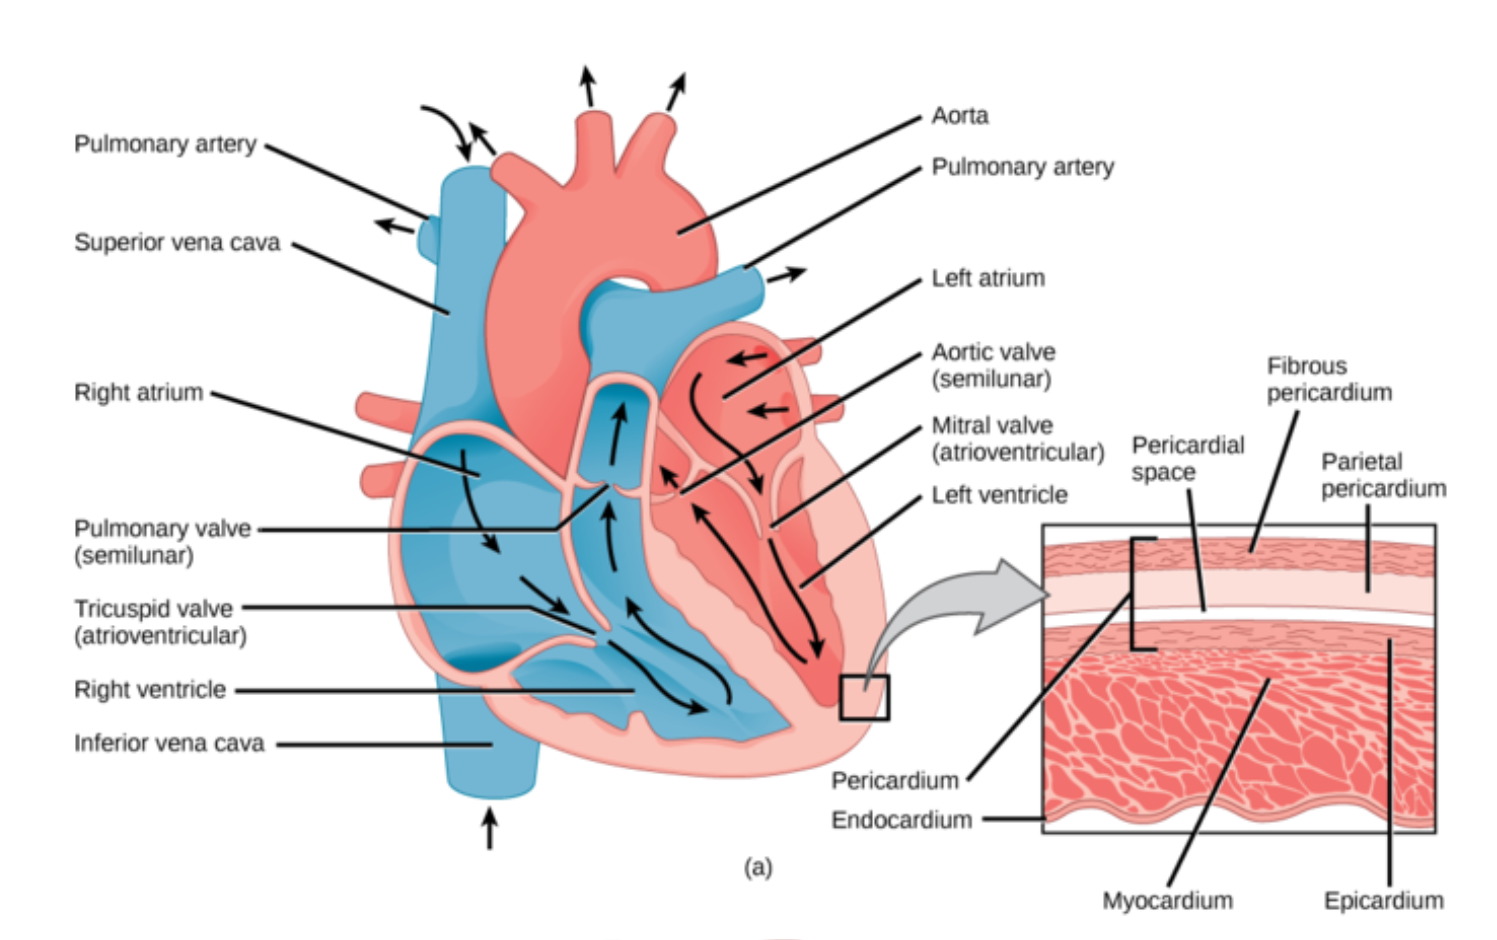
\includegraphics[width=50em]{heart}
	\end{center}
\begin{itemize}
	\item The above image has the ``left" in red.
	\item The paricardium encases the entire heard and produces a fluid into the sac to reduce friction.
		\begin{itemize}
			\item It has coranary arteries and cardiac veins all over it, supplying blood to the heart.
			\item These are subject to getting clogs, starving the heart of oxygen, making it necessary to get bippass surgery
			\item There are 4 coranary arteries, so to get all 4 fixed is calleed quadrupal bipass
			\item they take an artery from the leg and replace the issue area in the coranary arteriese.
				\begin{itemize}
					\item A small enough artery will be rebuilt after removal
				\end{itemize}
		\end{itemize}
	\item KNow the basic path: a figure 8
		\begin{itemize}
			\item 1. Lungs - oxygenated blood
			\item left atrium
			\item left ventricle
			\item aorta -- systemic cicuit -- $O_2$ used up
			\item Right atarium
			\item right ventricle
			\item back to lungs
		\end{itemize}
		\begin{center}
			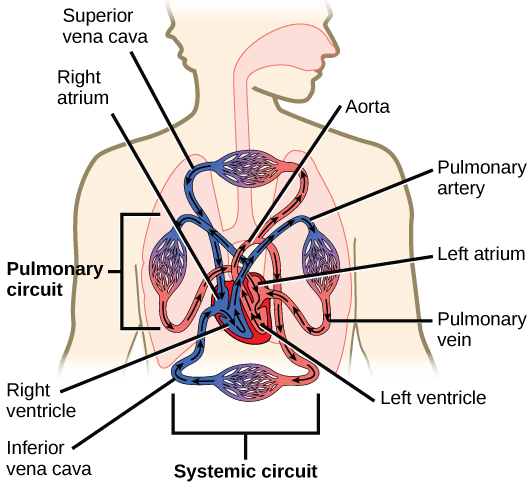
\includegraphics[width=50em]{bloodpath}
		\end{center}
	\item the heart beat is intrinsic -- it runs on its own
		\begin{itemize}
			\item specialized areas of cells  -- Nootes (SA and AV) -- coordinate the contraction/relaxation cycle, the big strong ``push" is when the venticular muscle contracts just after the spike in the ECG)
		\end{itemize}
\end{itemize}

\end{document}
